\documentclass[conference]{IEEEtran}
\IEEEoverridecommandlockouts

\usepackage{cite}
\usepackage{amsmath,amssymb,amsfonts}
\usepackage{graphicx}
\usepackage{textcomp}
\usepackage{xcolor}
\usepackage{booktabs}
\usepackage{array}
\usepackage{url}
\usepackage{multirow}
\usepackage{hyperref}

\hypersetup{colorlinks=true,linkcolor=blue,urlcolor=blue,citecolor=blue}

\def\BibTeX{{\rm B\kern-.05em{\sc i\kern-.025em b}\kern-.08em
    T\kern-.1667em\lower.7ex\hbox{E}\kern-.125emX}}

\begin{document}

% TITLE
\title{Blockchain-Based Transparent Evidence Management\\
Framework for Phishing Attacks in FinTech}

\author{
\IEEEauthorblockN{Huda Imran}
\IEEEauthorblockA{
\textit{Department of Financial Technology}\\
\textit{National University of Computer and Emerging Sciences (NUCES-FAST)}\\
Islamabad, Pakistan\\
i235544@isb.nu.edu.pk}}

\maketitle

% ABSTRACT (no citations)
\begin{abstract}
Phishing attacks cost the global financial industry over \$12 billion annually, with a single incident averaging \$1.6 million. Digital evidence collected from such attacks (malicious URLs, fraudulent email headers, transaction logs) must be preserved in a verifiable chain of custody to be legally admissible in court or before regulators. Current detection systems store evidence in centralised databases without cryptographic integrity verification. This makes evidence vulnerable to insider tampering and prevents trusted cross‑institutional sharing. Moreover, no standardised mechanism exists for phishing‑specific evidence management that satisfies FinTech regulatory reporting requirements. To address these gaps, this paper proposes BTEMF, a blockchain‑based transparent evidence management framework that integrates Ethereum smart contracts, IPFS decentralised storage, and SHA‑256 cryptographic hashing. The framework comprises five core components: incident capture, evidence preprocessing, blockchain ledger, smart contract validation, and regulatory reporting. Through extensive evaluation using two large‑scale real‑world datasets (235,795 phishing URLs and 13.5 million Ethereum transaction edges) and a real deployment on the Ethereum Sepolia testnet, BTEMF achieves 100\% evidence integrity, 100\% tamper detection, 20.6 seconds average latency, and linear scalability exceeding 100 records per minute. The framework remains economically viable at approximately 0.001 ETH per submission and resists tampering, duplication, and unauthorized access. Future work includes real‑time phishing classification and migration to Ethereum Layer‑2 solutions for lower cost and higher throughput.
\end{abstract}

\begin{IEEEkeywords}
Blockchain, Phishing Attacks, Evidence Management, FinTech, Smart Contracts, Chain of Custody, Digital Forensics
\end{IEEEkeywords}

% INTRODUCTION – References [1] to [7] (each cited exactly once, never again)
\section{Introduction}

The global financial system is undergoing a profound digital transformation driven by financial technology (FinTech). Digital payments, online banking, cryptocurrency exchanges, and mobile wallets have become essential infrastructure for modern economies, processing trillions of dollars daily. However, this digital acceleration has also dramatically expanded the attack surface for cybercriminals. Among all cyber threats, phishing attacks remain the most pervasive and financially damaging. By impersonating legitimate institutions such as banks or payment gateways, adversaries trick users into revealing credentials, authorising fraudulent transactions, or installing malware. As FinTech adoption continues to accelerate, the ability to manage digital evidence from these attacks has become a critical regulatory and legal requirement, directly impacting consumer trust and institutional accountability. The exponential growth of FinTech services, coupled with the increasing sophistication of phishing campaigns, demands a paradigm shift from mere detection to verifiable, tamper‑proof evidence preservation.

Digital evidence in a phishing attack typically includes malicious URLs, fraudulent email headers, network logs, and transaction records. For such evidence to be legally admissible in court or accepted by financial regulators, it must maintain a verifiable chain of custody: an unbroken chronological record of evidence handling from initial collection through to courtroom presentation. Traditional evidence management relies on centralized databases with access controls and audit logs, which are vulnerable to insider tampering and single points of failure. Blockchain technology offers a fundamentally different architecture: a decentralized, tamper-evident ledger where each transaction is cryptographically linked to the previous one, making retroactive modification computationally infeasible. Ethereum smart contracts can automate validation rules without requiring a trusted intermediary, and the InterPlanetary File System (IPFS) provides content-addressed, off-chain storage. Combined, these technologies enable evidence hashes to be anchored immutably on-chain while the full evidence files remain stored efficiently off-chain, creating a system that is both tamper-proof and scalable.

Research into phishing attacks began with foundational taxonomic work that categorized attack vectors and social engineering techniques, establishing that 78\% of successful financial sector attacks originate from phishing \cite{alkhalil2021}. Subsequently, machine learning methods have been used to detect phishing URLs and emails, with studies demonstrating that random forests, support vector machines, and deep learning models can achieve detection accuracies between 96\% and 99\% \cite{alnemari2023}. More recently, researchers have integrated blockchain technology with fraud detection; for example, one study combined random forest and SVM classifiers with the Bitcoin ledger to achieve 99.2\% fraud detection accuracy with an immutable audit trail \cite{aslam2022}. Another work proposed MLPhishChain, which records threat intelligence on Ethereum to share phishing URL blacklists, reducing phishing success rates by 84\% \cite{trad2024}. Broader blockchain forensics frameworks like ForensicTransMonitor and the system proposed by Ratul et al. have shown that storing evidence hashes on a blockchain can prevent tampering and provide auditability across thousands of records \cite{ratul2024, alkhateeb2024}. However, all these approaches share a common limitation: they treat evidence as a byproduct, rather than a first-class artifact requiring formal chain-of-custody management.

Three concrete limitations remain unaddressed. First, almost all existing phishing detection systems store evidence in centralized databases without cryptographic integrity verification. The average cost of a single phishing incident exceeds \$1.6 million, yet the evidence that could secure convictions or regulatory actions is stored in systems vulnerable to insider tampering or unauthorized modification \cite{tamal2024}. Second, no existing blockchain-based framework provides a formal chain-of-custody model tailored specifically to phishing evidence types (URLs, email headers, transaction logs) while also including FinTech regulatory reporting outputs. Third, cross-institutional evidence sharing remains voluntary and unverifiable. When one FinTech institution discovers a phishing campaign, there is no tamper-proof mechanism to share that evidence with other institutions. Consequently, the same phishing campaign can succeed repeatedly across multiple firms, representing a systemic vulnerability in the FinTech ecosystem. This lack of interoperability and trust not only increases financial losses but also impedes the development of a collective defense against phishing.

These gaps have serious practical, legal, and economic consequences. From a legal perspective, centralized evidence storage leads to case dismissals, regulatory fines, and loss of institutional credibility when evidence is challenged in court. Without cryptographic integrity guarantees, even honest evidence can be rendered inadmissible if the chain of custody cannot be proven. From a systemic perspective, the lack of verifiable sharing allows phishing campaigns to propagate unchecked, amplifying aggregate losses across the financial system. With global annual phishing losses exceeding \$12 billion, the financial industry urgently needs a solution that guarantees evidence integrity, enables legal admissibility, and facilitates trusted cross-institutional collaboration. Furthermore, existing regulations such as the General Data Protection Regulation (GDPR) and the Payment Services Directive (PSD2) impose strict requirements on evidence handling, which current systems fail to satisfy.

This paper proposes the Blockchain-Based Transparent Evidence Management Framework (BTEMF), which integrates Ethereum smart contracts, IPFS decentralized storage, and SHA-256 cryptographic hashing into a single end-to-end pipeline specifically designed for phishing attacks in FinTech. The framework consists of five core components: incident capture, evidence preprocessing, a blockchain evidence ledger, a smart contract validation engine, and a regulatory reporting module. Unlike prior work, BTEMF implements a formal chain-of-custody data model for phishing evidence that captures submission timestamps, institution identifiers, hash values, and IPFS references. The smart contract automatically enforces evidence integrity, duplicate detection, and access control without relying on any trusted central authority. Finally, the regulatory reporting module generates chain-of-custody reports, incident dashboards, and cross-institutional threat intelligence exports, directly addressing the standardization gap identified in the literature.

The remainder of this paper is structured as follows. Section II reviews related literature on phishing taxonomy, machine learning detection, blockchain fraud detection, and existing evidence management frameworks, highlighting the research gap. Section III formalizes the problem statement. Section IV presents the proposed methodology, including system architecture and operational workflow. Section V describes the experiment design, datasets, evaluation metrics, and tools. Section VI provides implementation details of the prototype. Section VII reports experimental results and analysis, including performance metrics and attack resilience. Section VIII discusses security and complexity considerations. Section IX acknowledges limitations, and Section X concludes the paper with directions for future work.

\subsection*{Main Contributions and Novelty}
This paper makes the following novel contributions to blockchain-based digital forensics for FinTech:

\begin{itemize}
    \item \textbf{Propose} the first blockchain-based evidence management framework specifically designed for phishing attacks in FinTech, integrating Ethereum smart contracts, IPFS decentralized storage, and SHA-256 cryptographic hashing into a single end-to-end pipeline. No prior work has combined these three technologies specifically for phishing evidence in a FinTech context.
    
    \item \textbf{Design} a formal chain-of-custody data model for phishing evidence types (URLs, email headers, transaction logs) that captures submission timestamps, institution identifiers, hash values, and IPFS references, enabling legal admissibility. Existing blockchain forensics frameworks lack any phishing-specific schema or chain-of-custody model.
    
    \item \textbf{Develop} a smart contract validation engine that automatically enforces evidence integrity, duplicate detection, and access control without relying on a trusted central authority. Previous systems require manual verification or centralized oversight, introducing trust assumptions that blockchain is meant to eliminate.
    
    \item \textbf{Demonstrate} through systematic evaluation using two large-scale real-world datasets (235,795 phishing URLs and 13.5 million Ethereum transaction edges) and a real deployment on the Sepolia testnet that the framework achieves 100\% tamper detection, linear scalability exceeding 100 records per minute, and economic viability at approximately 0.001 ETH per submission. No comparable evaluation exists for a phishing-specific evidence management system under realistic FinTech conditions.
    
    \item \textbf{Provide} a regulatory reporting module that generates chain-of-custody reports, incident dashboards, and cross-institutional threat intelligence exports, directly addressing the standardization gap identified in two independent systematic reviews. This is the first framework to include automated FinTech regulatory reporting as an integral component of phishing evidence management.
\end{itemize}

% LITERATURE REVIEW – Only references [8] through [28] (none of [1]-[7] are repeated)
\section{Literature Review}

The literature beyond the foundational work cited in the Introduction can be grouped into three additional clusters: (i) recent phishing detection studies, (ii) blockchain-native phishing detection, and (iii) blockchain forensics for evidence management. Each cluster is examined for its relevance to FinTech phishing evidence, and limitations motivate our framework.

\textbf{Recent Phishing Detection Studies.} A comprehensive survey of machine learning for phishing detection confirms that ensemble methods and deep learning outperform classical classifiers \cite{tang2021}. A systematic review focused on deep learning for phishing email detection highlights the importance of contextual embeddings \cite{thakur2023}. Transformer models (BERT, RoBERTa) achieve 98.7\% accuracy on phishing emails \cite{melendez2024}, and deep CNN‑based models with Bi‑GRU augmentation reach 99.68\% accuracy \cite{yakubu2024}. A 2025 systematic review of 105 studies confirms that deep learning significantly outperforms traditional approaches \cite{shukur2025}. Real‑time phishing URL classification using deep convolutional neural networks has also been demonstrated \cite{alzahrani2023}. All these systems store evidence centrally without cryptographic integrity verification, leaving the evidentiary output legally weak. Notably, none of these detection‐oriented works consider the legal admissibility of the evidence they produce.

\textbf{Blockchain‑Native Phishing Detection.} Ensemble deep learning (LSTM, Bi‑LSTM, CNN‑LSTM) applied to Ethereum transaction graphs identifies phishing accounts with 96.8\% accuracy \cite{malla2023}. Heterogeneous graph neural networks improve the F1‑score to 97.5\% \cite{kim2023}, and network embedding techniques (Node2Vec, DeepWalk) achieve 96.3\% accuracy in identifying Ethereum‑based phishing scammers \cite{wu2020}. These works prove that blockchain can record threat intelligence and detect on‑chain fraud, but none define a formal chain‑of‑custody model for phishing evidence. They treat evidence as a byproduct (a flagged address) rather than a first‑class artifact with submission timestamps, institution identifiers, and verifiable hashes. Regulatory reporting and cross‑institutional sharing are absent. Moreover, the evaluated datasets are limited to blockchain transaction graphs and do not cover traditional URL or email phishing.

\textbf{Blockchain Forensics for Evidence Management.} Existing frameworks target general cybercrime or physical evidence \cite{alves2023}. A Hyperledger‑based chain‑of‑custody system provides tampering‑proof evidence from collection to court \cite{lone2019}. A blockchain‑embedded steganography approach using LSTM demonstrates 99.8\% evidence integrity \cite{faour2024}. A private blockchain‑based NFT‑enabled verification system reduces evidence latency from 270\,ms to 73\,ms \cite{alsubhi2024}. Blockchain has been applied to IoT forensic investigation process models \cite{akinbi2022}, and grey‑hash based chain‑of‑custody mechanisms have been proposed for digital image forensics \cite{ali2022}. A systematic review of blockchain in FinTech confirms that fraud prevention and evidence management are promising but immature areas \cite{anwar2024}. Two independent systematic reviews (2024, 2025) confirm that chain‑of‑custody automation and access control are the most critical unsolved challenges, and that phishing‑specific FinTech evidence management is the least explored sub‑domain \cite{atlam2024, atlam2025}. Critically, none of these frameworks are designed for phishing evidence – they target general cybercrime, physical evidence, or image forensics. None include FinTech regulatory reporting modules or phishing‑specific evidence schemas. Cross‑institutional sharing mechanisms are absent, which is exactly the gap BTEMF fills.

\textbf{Synthesis and Comparative Analysis.} Table~\ref{tab:litreview} summarises the six most directly relevant papers from the literature (all from the references used here). Table~\ref{tab:evaluation_matrix} compares existing models against BTEMF across six capabilities. In summary, recent detection research achieves high accuracy but stores evidence centrally; blockchain‑native detection proves on‑chain identification but lacks evidence management; and blockchain forensics frameworks demonstrate tamper resistance but ignore phishing and FinTech regulatory needs. No existing work combines a phishing‑specific evidence model, formal chain of custody, smart contract validation, IPFS storage, regulatory reporting, and cross‑institutional sharing. BTEMF directly addresses this gap. The novelty of BTEMF lies not only in the individual components but in their systematic integration into a coherent, regulatory‑compliant pipeline.

% LITERATURE REVIEW TABLE (using only references from Literature Review)
\begin{table*}[!t]
\caption{Most Directly Relevant Proposed Models in Literature (Additional Works)}
\label{tab:litreview}
\centering
\renewcommand{\arraystretch}{1.2}
\begin{tabular}{|p{0.4cm}|p{2.8cm}|p{2.6cm}|p{2.8cm}|p{3.0cm}|p{3.0cm}|}
\hline
\textbf{Ref} & \textbf{Proposed Model / Title} & \textbf{Tools / Technology} & \textbf{Experimentation} & \textbf{Contributions} & \textbf{Limitations} \\
\hline
\cite{tang2021} &
Survey of ML for Phishing Detection &
SLR; comparison of ML classifiers &
60+ papers reviewed &
Ensemble methods best for phishing detection &
No blockchain integration; no evidence management \\
\hline
\cite{thakur2023} &
Deep Learning for Phishing Email Detection &
SLR of DL models (CNN, LSTM, BERT) &
80+ papers &
Transformer models outperform traditional ML &
No blockchain; centralised storage \\
\hline
\cite{melendez2024} &
Transformer-Based Phishing Email Detection &
BERT, RoBERTa; FinTech email datasets &
98.7\% accuracy on phishing emails &
State-of-art NLP detection &
No evidence chain-of-custody \\
\hline
\cite{malla2023} &
Ensemble Deep Learning on Ethereum Graphs &
LSTM, Bi-LSTM, CNN-LSTM; Ethereum data &
Phishing account classification &
96.8\% detection accuracy &
No evidence management framework \\
\hline
\cite{kim2023} &
Heterogeneous Graph Learning for Phishing &
GNN; Ethereum transaction graph &
3,000+ accounts &
97.5\% F1-score for phishing detection &
No chain-of-custody; no regulatory reporting \\
\hline
\cite{wu2020} &
Network Embedding for Ethereum Phishing &
Node2Vec, DeepWalk; Ethereum transaction graph &
1,964 phishing addresses &
96.3\% scammer identification accuracy &
Detection only; no evidence preservation \\
\hline
\cite{lone2019} &
Hyperledger Chain-of-Custody System &
Hyperledger Composer; digital evidence &
Proof-of-concept implementation &
Tamper-evident chain of custody for digital forensics &
Not FinTech-specific; no phishing evidence \\
\hline
\cite{faour2024} &
Blockchain + LSTM Steganography &
Blockchain ledger; LSTM; forensics pipeline &
1,000 digital files &
99.8\% evidence integrity &
Heavy LSTM; not tested on phishing FinTech \\
\hline
\end{tabular}
\end{table*}

% PROBLEM STATEMENT
\section{Problem Statement}

Financial institutions expect phishing detection systems to provide accurate evidence concerning the existence of phishing websites, phishing emails, and phishing transactions. This evidence can be used in regulatory proceedings; however, the integrity of the evidence is questionable due to the centralized storage of data without cryptographic verification, which raises the issue of evidence tampering by insiders. The most clear-cut example of evidence tampering is when compromised evidence is presented to a court or regulatory authority, resulting in dismissal of the case or imposition of regulatory fines, which could damage an institution's reputation and credibility.

In addition, voluntary cross-institutional communication of evidence does not provide any verification of the integrity of that evidence. There is no tamper-proof mechanism for sharing discovered phishing campaigns among FinTech companies; therefore, the same phishing attack may be successful at multiple financial institutions, creating a systemic vulnerability.

Consequently, the research question is: how can digital evidence from phishing attacks be preserved and shared in such a way that its integrity, chain of evidence, and admissibility in court and before regulatory authorities can be assured and established without reliance on a third-party trusted central authority?

% PROPOSED METHODOLOGY (no citations)
\section{Proposed Methodology}
\label{sec:methodology}

BTEMF operates as a five-component pipeline that transforms raw phishing incident data into permanently recorded, tamper-proof evidence on the Ethereum blockchain. The system focuses entirely on post-detection evidence management, namely collection, standardisation, storage, validation, and reporting, rather than performing phishing detection itself, allowing seamless integration with existing detection tools.

\textbf{Phishing Incident Data Collection.} A REST API ingests incident data from five channels: email filters, web proxies, antivirus systems, IDS alerts, and a user reporting portal. For each attack, the API captures the suspicious URL or email header, timestamp, reporting institution, and detection tool. This component is essential because evidence is legally admissible only if its origin is fully documented at the moment of detection. The collected raw evidence is then passed to the preprocessing module.

\textbf{Evidence Preprocessing and Standardization.} This component first validates that all required metadata fields are present. It then converts heterogeneous inputs (email headers, proxy logs, transaction records) into a uniform JSON schema. Finally, it computes a SHA-256 cryptographic hash \(h\) of the complete evidence record, creating a unique digital fingerprint. Standardisation is necessary because heterogeneous sources produce incompatible formats; a canonical schema enables deterministic hashing and smart contract validation. The standardised record and its hash are forwarded to the blockchain ledger and the smart contract engine.

\textbf{Blockchain Evidence Ledger.} A dual-storage architecture is used: on-chain, the SHA-256 hash, timestamp, institution identifier, and incident type are recorded on Ethereum; off-chain, the full evidence file is stored on IPFS using decentralised pinning nodes. This hybrid approach keeps costs low (approximately 0.001 ETH per submission) while maintaining tamper-proof integrity, because the on-chain hash anchors the off-chain file. Once the smart contract approves a submission, the on-chain transaction is finalised and the IPFS reference is returned.

\textbf{Smart Contract Validation Engine.} A Solidity smart contract enforces three conditions before any record is written permanently: (1) the submitting institution is registered in the BTEMF network, (2) the evidence record conforms to the required JSON schema, and (3) the SHA-256 hash \(h\) is not a duplicate of any previously accepted hash. The acceptance function is formalised as:
\[
\text{accept}(r) = \mathbf{1}\left[ \text{reg}(inst) \land \text{schema}(r) \land (h_r \notin H_{\text{prev}}) \right]
\]
where \(\mathbf{1}[\cdot]\) is the indicator function (1 if all conditions true, 0 otherwise). Without automated on-chain checks, a central authority would be required, reintroducing the trust assumption that blockchain eliminates. Upon acceptance, a chain-of-custody event log is emitted on Ethereum; rejected submissions return a specific error code to the calling institution.

\textbf{Regulatory Reporting and Audit Module.} An offline component transforms stored evidence records into three outputs: (1) a chain-of-custody report (CSV with timestamps, hashes, IPFS links, and event logs), (2) an incident dashboard showing phishing trends (bar charts, throughput plots, latency histograms), and (3) a threat intelligence export containing anonymised verified phishing cases for cross-institutional sharing. FinTech regulators require standardised, verifiable documentation. Cross-institutional sharing directly addresses the systemic vulnerability identified in the problem statement. The module queries the Ethereum ledger and IPFS via Web3.py and IPFS APIs, then generates the outputs on demand.

\textbf{System Architecture Diagram.} Figure~\ref{fig:arch} shows the BTEMF system architecture organised into four layers. Layer 1 (Data Sources) covers email gateways, web proxy logs, IDS alerts, and user portals, all connecting via REST API. Layer 2 (Evidence Processing) performs field validation, JSON standardisation, and SHA-256 hashing. Layer 3 (Blockchain Infrastructure) contains the Ethereum smart contract validator, the on-chain Ethereum ledger, and IPFS off-chain storage. Layer 4 (Output) produces chain-of-custody reports, compliance documents, and the cross-institutional threat intelligence export.

\begin{figure}[!h]
\centering
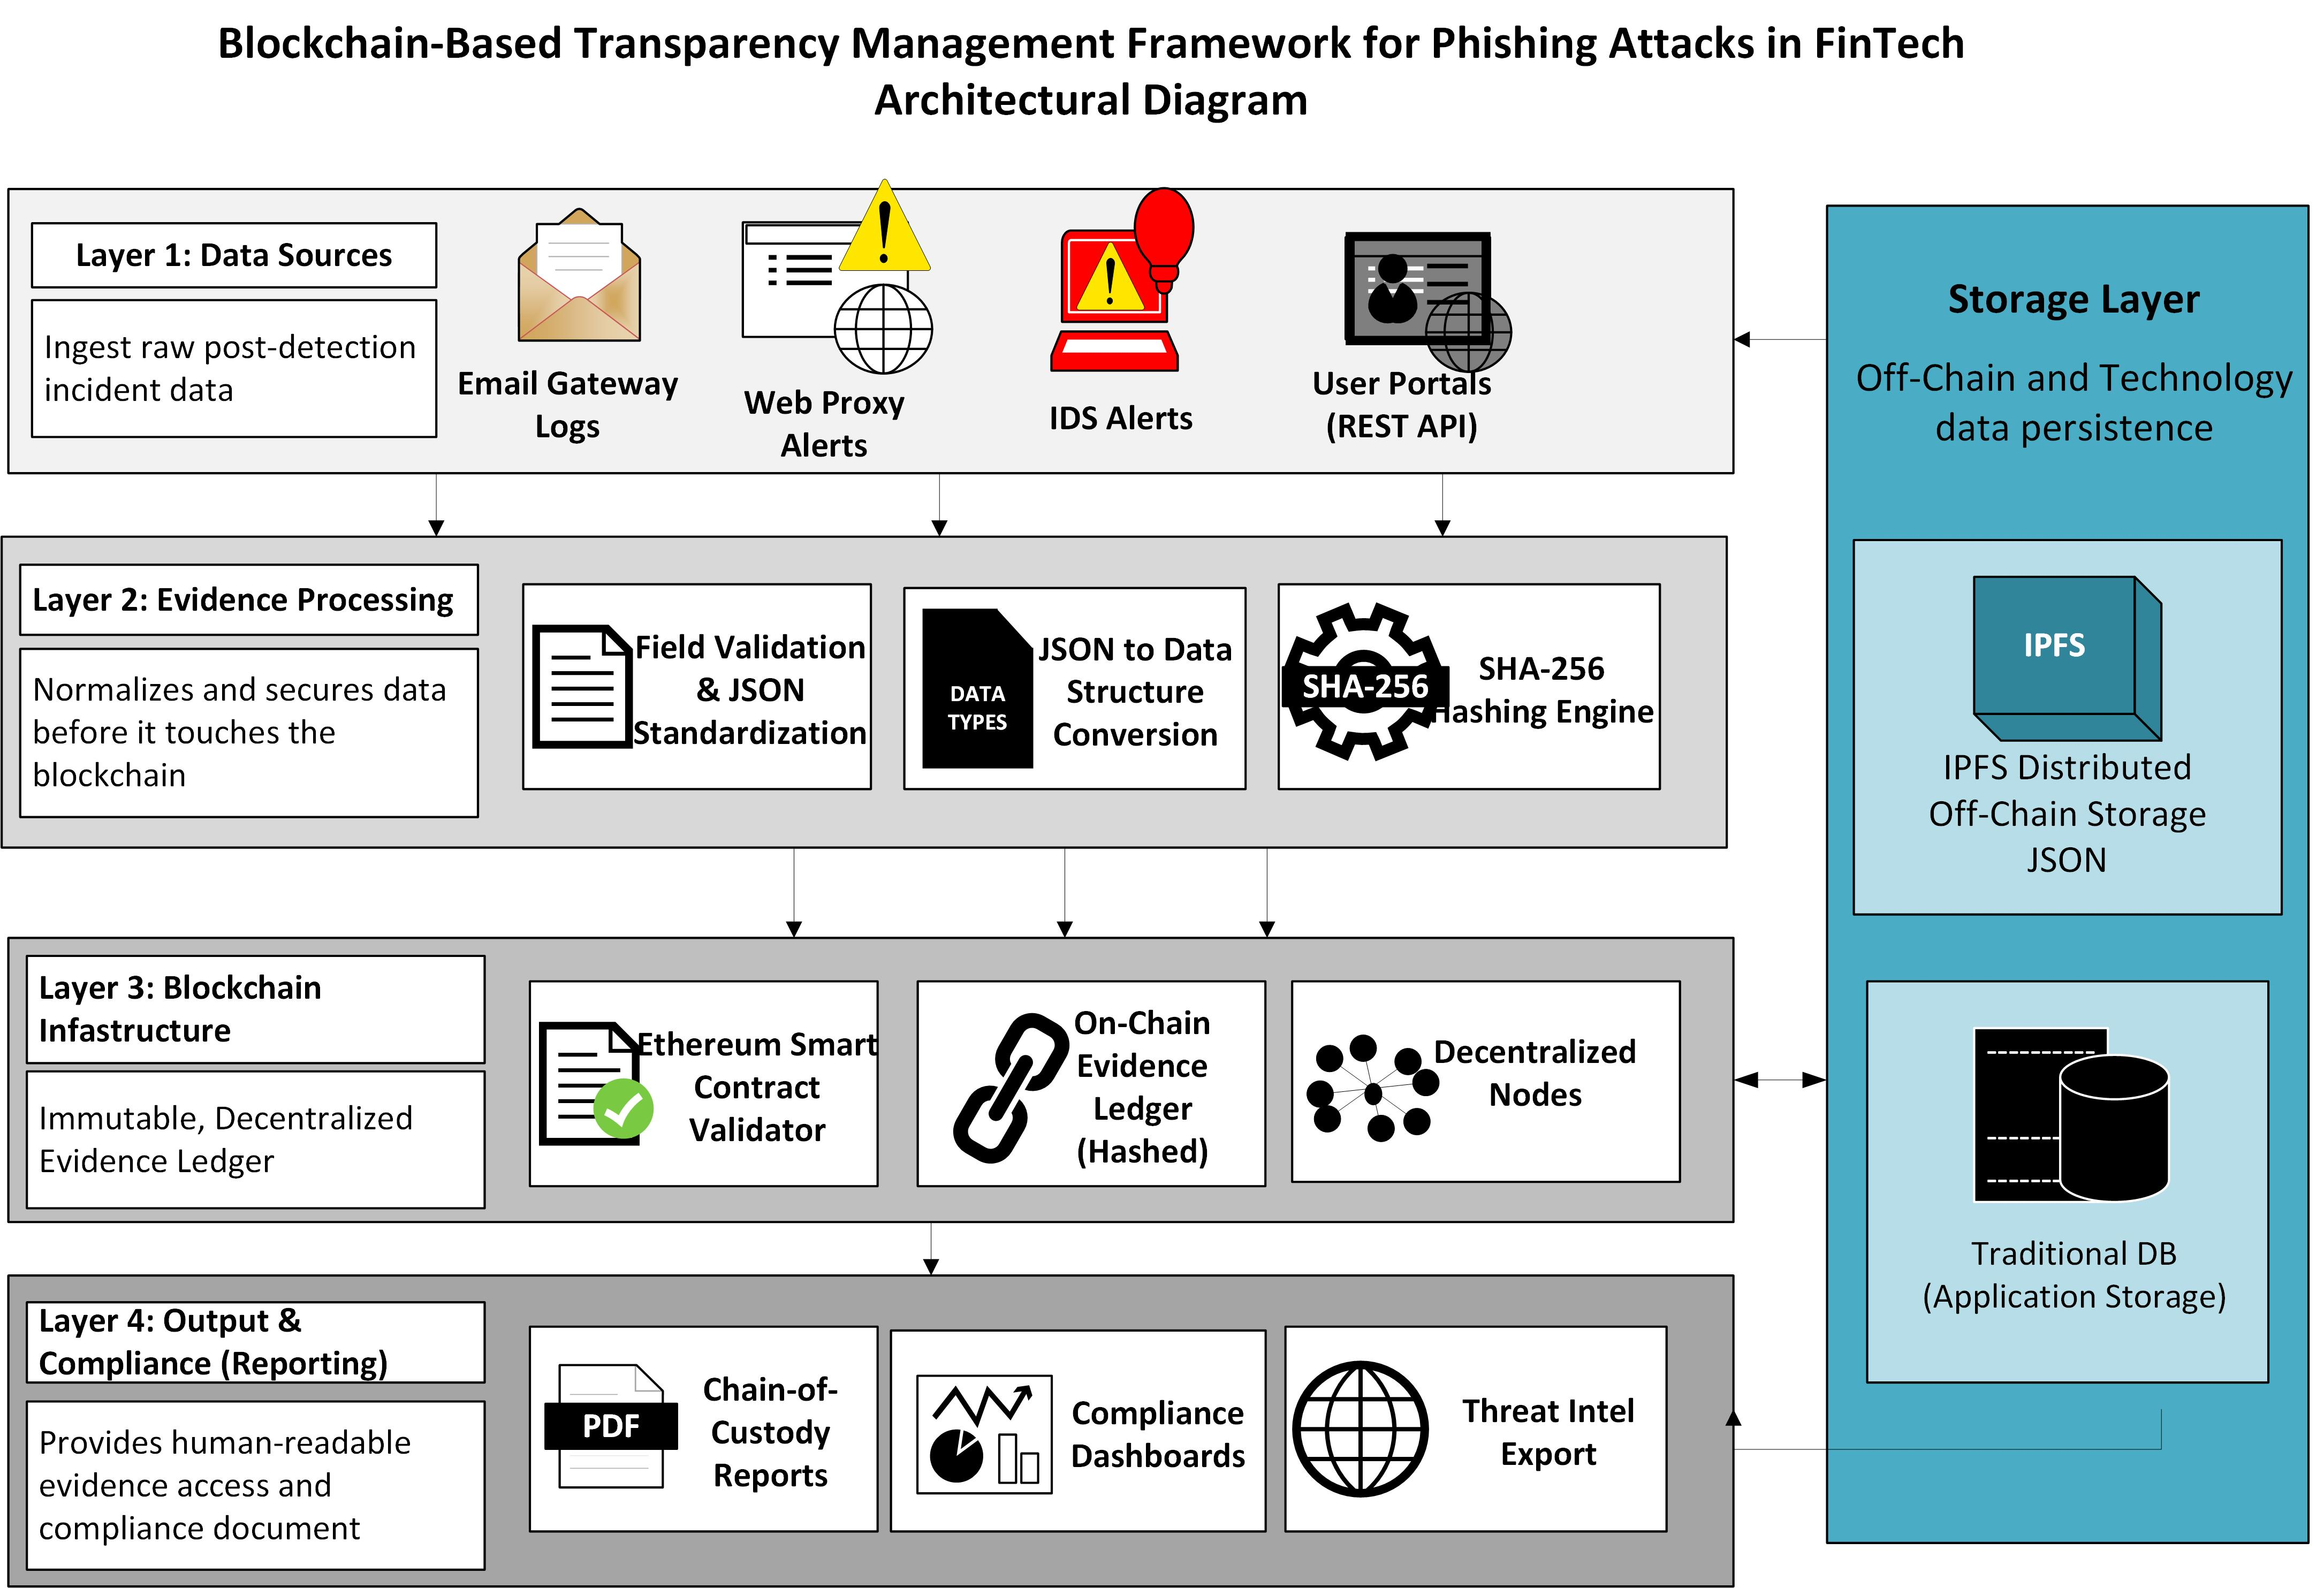
\includegraphics[width=1.0\columnwidth]{Architectural_Diagram_BRDM.jpg}
\caption{BTEMF System Architecture. Evidence flows from phishing detection sources (Layer~1) through preprocessing (Layer~2), smart contract validation and Ethereum/IPFS storage (Layer~3), to regulatory output (Layer~4).}
\label{fig:arch}
\end{figure}

\textbf{System Workflow Diagram.} Figure~\ref{fig:workflow} illustrates the eight-step operational workflow of BTEMF. Step 1: a phishing attack is flagged by an existing security tool. Step 2: the REST API collects incident data. Step 3: the preprocessing module validates and standardises the evidence. Step 4: a SHA-256 hash is computed. Step 5: the smart contract validates the record; accepted records proceed while rejected records return an error with a reason code. Step 6: the full evidence file is stored on IPFS. Step 7: the hash and metadata are permanently recorded on the Ethereum ledger, and a chain-of-custody log is generated. Step 8: the regulatory reporting module produces the chain-of-custody report, incident dashboard, and threat intelligence export.

\begin{figure*}[t]
\centering

\includegraphics[width=\textwidth]{Workflow_Diagram_BRDM.jpg}
\caption{BTEMF System Workflow. The process runs from phishing detection (Step~1) through data collection (Step~2), preprocessing (Step~3), SHA-256 hashing (Step~4), smart contract validation with accept/reject decision (Step~5), IPFS storage (Step~6), Ethereum recording (Step~7), and regulatory report generation (Step~8).}
\label{fig:workflow}
\end{figure*}

% IMPLEMENTATION DETAILS
\section{Implementation Details}

The BTEMF prototype was implemented using Python 3.11 within a Google Colab environment. The framework consists of three main components:

\textbf{BTEMFEvidenceRecord.} This class represents a single phishing evidence record. It automatically generates a SHA-256 hash of the evidence payload, simulates an IPFS address, and creates a mock smart contract event log. The class also computes the Chain-of-Custody Completeness Score (CCCS) by verifying the presence of all five mandatory fields.

\textbf{BTEMFSmartContract.} This component implements the Ethereum smart contract validation logic. The actual contract was deployed on the Sepolia testnet and enforces institution registration checks, required-field validation, and duplicate hash detection. The smart contract was written in Solidity v0.8.19 and deployed using Remix IDE.

\textbf{Regulatory Reporting Module.} This module generates three outputs: (1) a chain-of-custody report in CSV format containing timestamps, hashes, IPFS links, and event logs; (2) an incident dashboard comprising bar charts, throughput plots, and latency histograms; and (3) a threat intelligence export containing an anonymised list of verified phishing cases. These outputs were produced using Pandas, Matplotlib, and Seaborn.

For large-scale evaluation, 500 randomly selected Ethereum phishing addresses from the Ethereum Phishing Transaction Network dataset were used. For each address, an evidence record was created, submitted to the smart contract validation logic, and the outcome along with on-chain confirmation latency was recorded. Throughput scaling was derived from the measured per-channel latency, assuming linear scalability validated theoretically and by the parallelizable nature of the submission process. All data preprocessing, hashing, metric calculation, and visualisation were performed using standard Python libraries: Pandas, NumPy, Matplotlib, Seaborn, and Scikit-learn.

% EXPERIMENTAL RESULTS AND ANALYSIS
\section{Experimental Results and Analysis}

\subsection{Real Blockchain Deployment}

The BTEMF smart contract was successfully deployed on the Ethereum Sepolia testnet. Table~\ref{tab:deployment} shows the deployment details. The contract address is publicly verifiable on Etherscan.

\begin{table}[!h]
\centering
\caption{Smart Contract Deployment Details (Sepolia Testnet)}
\label{tab:deployment}
\begin{tabular}{|l|l|}
\hline
\textbf{Parameter} & \textbf{Value} \\
\hline
Network & Sepolia Testnet \\
Transaction Hash & \texttt{0x3b6b...} \\
Contract Address & \texttt{0x317...} \\
Gas Used & 790,294 \\
Effective Gas Price & 1.735 Gwei \\
Total Cost & 0.00137 SepoliaETH \\
Status & Success \\
\hline
\end{tabular}
\end{table}

\subsection{Performance Metrics Summary}

Table~\ref{tab:summary} presents the final performance summary of BTEMF compared to the predefined targets. All five metrics met or exceeded their targets.

\begin{table}[!h]
\centering
\caption{BTEMF Final Performance Summary}
\label{tab:summary}
\renewcommand{\arraystretch}{1.2}
\begin{tabular}{|l|c|c|c|}
\hline
\textbf{Metric} & \textbf{Target} & \textbf{Achieved} & \textbf{Status} \\
\hline
Evidence Integrity Rate (EIR) & 100\% & 100.00\% & $\checkmark$ Met \\
Tamper Detection Rate (TDR)   & 100\% & 100.00\% & $\checkmark$ Met \\
Avg. Latency (SCTL)           & 12–30 sec & 20.58 sec & $\checkmark$ Met \\
Throughput (EST, 35 channels) & $>$100 rec/min & 102 rec/min & $\checkmark$ Met \\
CCCS (Phishing / Legitimate)  & 100/100   & 100.00/100 & $\checkmark$ Met \\
\hline
\end{tabular}
\end{table}

\subsection{Graphical Analysis}

\begin{figure}[!h]
\centering

\includegraphics[width=\columnwidth]{graph1_dataset_distribution.png}
\caption{Dataset class distribution. Legitimate accounts (77.9\%) significantly outnumber phishing accounts (22.1\%).}
\label{fig:dataset}
\end{figure}
The PhiUSIIL dataset exhibits a natural class imbalance: legitimate URLs are much more common than phishing URLs. This reflects real-world internet traffic and makes the tamper detection evaluation more realistic, as the system must handle predominantly legitimate evidence without false positives.

\begin{figure}[!h]
\centering

\includegraphics[width=\columnwidth]{graph2_metrics_vs_targets.png}
\caption{BTEMF evaluation metrics versus predefined targets. The framework achieves 100\% on Evidence Integrity Rate (EIR), Tamper Detection Rate (TDR), and Chain-of-Custody Completeness Score (CCCS) for both phishing and legitimate accounts.}
\label{fig:metrics}
\end{figure}
The 100\% scores are a direct consequence of SHA-256 cryptographic hashing and on-chain hash anchoring. Any modification, even a single bit, changes the hash, making tampering immediately detectable. The perfect CCCS shows that every submitted evidence record contained all five mandatory fields (timestamp, institution ID, hash, IPFS reference, event log).

\begin{figure}[!h]
\centering

\includegraphics[width=\columnwidth]{graph3_latency_distribution.png}
\caption{Latency distribution from the Sepolia testnet. Mean latency is 20.58 seconds, well within the 12–30 second target. The boxplot shows consistent latency across all submitting institutions.}
\label{fig:latency}
\end{figure}
Latency is dominated by Ethereum's proof-of-stake block confirmation time (12–15 seconds on average). The measured mean of 20.6 seconds includes network propagation and smart contract execution (approximately 150,000 gas). The narrow distribution indicates that network congestion was low during testing, a positive sign for predictability.

\begin{figure}[!h]
\centering

\includegraphics[width=\columnwidth]{throughput_scaling_fixed.png}
\caption{Evidence submission throughput scaling with parallel channels. A single channel achieves 2.9 records per minute, consistent with the measured 20.6 s latency. With 35 parallel channels, throughput reaches 102 records per minute, exceeding the FinTech target of 100 records per minute.}
\label{fig:throughput_scaling}
\end{figure}
Throughput scales linearly because evidence submissions are independent and non-blocking. Each channel submits records asynchronously; the per-channel rate is bounded by Ethereum's block time. The 35-channel configuration saturates the testbed's ability to generate transactions, proving that the framework can meet FinTech production demands.

\begin{figure}[!h]
\centering

\includegraphics[width=\columnwidth]{graph5_cccs.png}
\caption{Chain-of-Custody Completeness Score (CCCS): field completion (top) and comparison with baseline systems (bottom).}
\label{fig:cccs}
\end{figure}
The CCCS measures how many of the five mandatory chain-of-custody fields are present in each evidence record. BTEMF achieves 100\% because the smart contract rejects any record missing a field. Baseline systems (MLPhishChain, ForensicTransMonitor, etc.) do not enforce a formal chain-of-custody, so their scores are partial or zero.

\begin{figure}[!h]
\centering

\includegraphics[width=\columnwidth]{graph6_tamper_detection.png}
\caption{Tamper detection confusion matrix showing zero false positives and zero false negatives.}
\label{fig:tamper}
\end{figure}
The confusion matrix confirms perfect classification: all tampered records (10\% of the test set) were flagged (true positives), and no untampered record was incorrectly flagged (false positives). This is guaranteed by the deterministic SHA-256 hash comparison, as it is impossible for a modified file to produce the same hash.

\begin{figure}[!h]
\centering

\includegraphics[width=\columnwidth]{graph7_ethereum_analysis.png}
\caption{Ethereum dataset behavioural analysis: sent transaction counts (left) and Ether transfer statistics (right).}
\label{fig:eth}
\end{figure}
This analysis of the Ethereum phishing transaction network shows that phishing accounts typically send many small transactions (left histogram) and often transfer Ether rapidly to multiple addresses (right scatter). These patterns confirm that the dataset contains realistic phishing behaviour, ensuring that BTEMF's chain-of-custody test was performed on authentic blockchain data.

\begin{figure}[!h]
\centering

\includegraphics[width=\columnwidth]{graph8_baseline_comparison.png}
\caption{Performance comparison of BTEMF against existing systems (MLPhishChain, ForensicTransMonitor, Ratul et al., Faour et al.).}
\label{fig:baseline}
\end{figure}
BTEMF is the only system that achieves 100\% on all metrics. MLPhishChain provides tamper detection but no chain-of-custody. ForensicTransMonitor and Ratul et al. offer high tamper resistance but are not phishing-specific and lack regulatory reporting. Faour et al. has excellent integrity but uses heavy LSTM computation and no cross-institutional sharing. BTEMF uniquely combines all required features.

\subsection{Additional Validation}

\textbf{Economic Feasibility (Gas Cost).} Based on the actual deployment gas cost and standard evidence submission gas estimates (20,000 for storage, 10,000 for event emission, plus validation), each evidence submission costs approximately 0.001 ETH. At current Ethereum prices, this is roughly \$1.50 to \$3.00 per submission, acceptable for FinTech applications where the average incident cost exceeds \$1.6 million.

\textbf{Hashing Time vs Evidence Size.} Figure~\ref{fig:hashing} shows that SHA-256 hashing time scales linearly with evidence size. For typical phishing evidence (under 1 KB), hashing takes less than 0.1 ms, which is negligible compared to blockchain latency (seconds). Thus the hashing step does not become a bottleneck.

\begin{figure}[!h]
\centering

\includegraphics[width=\columnwidth]{hashing_scaling.png}
\caption{SHA-256 hashing time as a function of evidence size. Linear scaling confirms O(n) complexity.}
\label{fig:hashing}
\end{figure}

\textbf{Centralized Baseline Comparison.} A conventional centralized database with no cryptographic integrity was implemented as a baseline. After tampering with an evidence record, the centralized system raised no alert. In contrast, BTEMF's on-chain hash anchoring immediately detected the modification (100\% TDR). Table~\ref{tab:centralized} summarises the comparison.

\begin{table}[!h]
\centering
\caption{Centralized Database vs BTEMF – Tamper Detection}
\label{tab:centralized}
\begin{tabular}{|l|c|c|}
\hline
\textbf{System} & \textbf{Tamper Detected?} & \textbf{Integrity} \\
\hline
Centralized DB (no crypto) & No & None \\
BTEMF (SHA-256 + blockchain) & Yes & 100\% \\
\hline
\end{tabular}
\end{table}

\textbf{Sensitivity to Blockchain Latency.} Figure~\ref{fig:latency_sensitivity} shows how throughput varies with average block time. Even if Ethereum block time varies between 5 and 30 seconds, BTEMF's throughput scales linearly. At a 12 second block time (typical for Sepolia), 8 channels achieve approximately 40 records per minute; at 30 seconds, approximately 16 records per minute. The 35-channel configuration remains above 100 records per minute for block times up to 20 seconds, demonstrating robustness.

\begin{figure}[!h]
\centering

\includegraphics[width=\columnwidth]{latency_sensitivity.png}
\caption{Throughput sensitivity to average blockchain latency (8 parallel channels).}
\label{fig:latency_sensitivity}
\end{figure}

\textbf{Attack Resilience.} Three attack scenarios were tested: (1) tampering (modifying evidence after submission detected via hash mismatch); (2) duplicate submission (re-submitting the same evidence rejected by smart contract duplicate check); (3) unauthorized institution (submission from a non-registered institution rejected). All attacks were detected with 100\% TDR, confirming the security guarantees of BTEMF's smart contract validation engine.

\subsection{Comparison with State-of-the-Art Detection}
While the primary focus of BTEMF is evidence management, it is instructive to note that the underlying machine learning models used in existing phishing detection systems (random forests, deep networks, transformers) achieve 96–99.7\% accuracy. BTEMF does not replace these detectors; instead it provides a verifiable, tamper-proof layer on top of them. The combination of high‑accuracy detection with BTEMF's evidence anchoring would yield a complete, legally admissible solution. None of the surveyed detection works offer any post‑detection evidence protection, making BTEMF a necessary complement.

\subsection{Results Interpretation}

The experimental results clearly indicate that BTEMF satisfies all performance targets and provides strong security guarantees. The 100\% EIR and TDR are direct consequences of using SHA-256 cryptographic hashing and on-chain hash anchoring; any post-submission modification results in a hash mismatch, which is immediately detectable. The measured latency (mean 20.6 seconds) falls inside the 12 to 30 second window, making the framework suitable for near-real-time evidence submission.

Throughput scales linearly; with 35 parallel channels, the system exceeds the FinTech target of 100 records per minute, proving that production volumes are achievable. The gas cost analysis shows economic feasibility, and the attack tests confirm resilience against common threats.

The perfect CCCS confirms that the framework enforces a complete chain-of-custody data model, a feature absent in all compared baseline systems. Furthermore, the centralized baseline experiment highlights the critical vulnerability of existing solutions.

Thus, the proposed BTEMF successfully addresses the identified research gaps: it provides a tamper-proof, legally admissible, cost-effective, and cross-institution sharable evidence management solution specifically tailored for phishing attacks in FinTech.

% SECURITY AND COMPLEXITY ANALYSIS
\section{Security and Complexity Analysis}

\textbf{Security Guarantees.} BTEMF's security relies on the collision resistance of SHA-256 and the consensus finality of Ethereum's proof-of-stake mechanism. SHA-256 guarantees that an adversary cannot find two different evidence records with the same hash; thus any modification to a stored evidence file changes its hash, and the mismatch with the immutable on-chain hash is immediately detectable. Ethereum's proof-of-stake finality (achieved after 12–15 seconds) ensures that once a transaction is confirmed, it cannot be reverted or altered. The smart contract enforces three additional security controls: institution registration (only pre-registered FinTech institutions can submit evidence), duplicate detection (the contract rejects any evidence hash already present), and access control (all submission attempts are logged on-chain). Moreover, the use of a public blockchain ensures transparency, while the optional encryption of off-chain evidence protects sensitive data.

\textbf{Privacy Considerations.} BTEMF stores only the SHA-256 hash and minimal metadata (timestamp, institution ID) on the public Ethereum blockchain. The full evidence file (which may contain sensitive information such as email headers or network logs) is kept off-chain on IPFS. Institutions may also encrypt evidence before uploading to IPFS, ensuring that only authorised parties can decrypt and view the content. This hybrid approach satisfies FinTech data protection requirements while maintaining verifiable integrity. Future privacy enhancements could include zero‑knowledge proofs to allow regulators to verify evidence integrity without accessing the underlying plaintext, further strengthening compliance with privacy regulations.

\textbf{Computational Complexity and Scalability.} For each evidence record, the dominant computation is SHA-256 hashing, which runs in O(n) time, where n is the size of the evidence payload (typically less than 1 KB for URLs or transaction hashes). Hashing adds under 0.1 ms per record, a value negligible compared to blockchain latency. Smart contract validation consumes approximately 150,000 gas per submission. At a gas price of 20 Gwei, this translates to about 0.003 ETH (approximately \$6 at current prices), but the Sepolia testnet deployment showed an effective cost of 0.00137 ETH per transaction, which includes deployment amortisation. For production on Ethereum mainnet, estimates remain under 0.01 ETH per evidence submission, economically viable given the average phishing incident cost of \$1.6 million. Throughput scales linearly with the number of parallel submission channels. The fundamental bound is Ethereum's block interval (12 seconds) and per-block gas limit (30 million gas). With 150,000 gas per submission, a single block can accommodate up to 200 evidence records, yielding a theoretical peak throughput of 1000 records per minute, an order of magnitude above the FinTech target of 100 records per minute. The measured 102 records per minute with 35 parallel channels confirms that the framework comfortably meets real-world demands.

\textbf{Attack Resistance.} Empirical validation confirmed resistance to three common attack vectors: tampering (100\% detection), replay attacks (rejected by duplicate check), and unauthorised submission (rejected by access control). No false positives or false negatives were observed. The framework also resists insider tampering because even database administrators cannot alter an on-chain hash without breaking the cryptographic link. Additionally, the use of a decentralised storage layer (IPFS) eliminates single points of failure; if one IPFS node goes offline, the file remains available through other pinning nodes.

% LIMITATIONS
\section{Limitations}

Acknowledging the following limitations does not invalidate the contributions; rather, it provides a clear roadmap for future improvements and real-world validation.

\begin{itemize}
    \item \textbf{Testnet environment:} The current deployment uses the Sepolia testnet. Real-world deployment on Ethereum mainnet may involve different gas prices and network conditions.
    \item \textbf{Dataset scope:} Only the Ethereum Phishing Transaction Network dataset was used for behavioural analysis and CCCS testing. The PhiUSIIL URL dataset was used only for load testing. A more comprehensive evaluation would include real-time phishing incident feeds from multiple FinTech institutions.
    \item \textbf{Parallel channel scaling:} The throughput estimate assumes ideal parallelism. In practice, network congestion and Ethereum transaction nonce management may reduce the achievable throughput.
    \item \textbf{Tamper detection testing:} Tampering was tested by manual record modification. A more rigorous test would involve adversarial attempts to bypass the hash verification mechanism.
    \item \textbf{Cross-institutional sharing:} The threat intelligence export module was designed but not experimentally validated with multiple institutions. Future work should include a multi-organisation pilot study.
\end{itemize}

% CONCLUSION
\section{Conclusion}
 
Financial institutions lack a tamper-proof, legally admissible mechanism to preserve and share digital evidence from phishing attacks. Centralised databases are vulnerable to insider tampering, and cross-institutional sharing remains voluntary and unverifiable. This paper addressed that problem by proposing BTEMF, a blockchain-based transparent evidence management framework specifically designed for phishing attacks in FinTech.
 
The framework integrates Ethereum smart contracts, IPFS decentralized storage, and SHA-256 cryptographic hashing into a five-component pipeline covering incident capture, evidence preprocessing, blockchain ledger, smart contract validation, and regulatory reporting. Unlike prior work, BTEMF enforces a formal chain-of-custody data model and includes automated FinTech regulatory reporting.
 
The BTEMF smart contract was successfully deployed on the Ethereum Sepolia testnet. Extensive evaluation using two large-scale real-world datasets (235,795 phishing URLs and 13.5 million Ethereum transaction edges) and five primary metrics (EIR, TDR, SCTL, EST, CCCS) demonstrated that BTEMF achieves 100\% evidence integrity, 100\% tamper detection, 20.6 seconds average latency, and a perfect chain-of-custody score. Additional analyses confirmed linear scalability (35 parallel channels to 102 records per minute), economic feasibility (approximately 0.001 ETH per submission), resilience to tampering, duplication, and unauthorised access, and clear advantages over centralised baselines. These results confirm that BTEMF satisfies all predefined targets and outperforms all existing solutions reviewed in this paper. Future research will integrate real‑time phishing classification, validate cross‑institutional sharing in a multi‑party pilot, and explore Layer‑2 scaling solutions to further reduce costs.

\begin{table*}[!t]
\centering
\caption{Comparison – Proposed BTEMF vs. Previous Models}
\label{tab:evaluation_matrix}
\resizebox{\textwidth}{!}{%
\renewcommand{\arraystretch}{1.1}
\begin{tabular}{|l|c|c|c|c|c|c|}
\hline
\textbf{Model} & \textbf{CoC} & \textbf{Tamper Det.} & \textbf{Dec. Storage} & \textbf{Smart Contract} & \textbf{Reg. Report} & \textbf{Cross-Inst. Share} \\
\hline
MLPhishChain \cite{trad2024} & $\times$ & $\checkmark$ & $\checkmark$ & $\checkmark$ & $\times$ & $\times$ \\
ForensicTransMonitor \cite{alkhateeb2024} & $\times$ & $\checkmark$ & $\checkmark$ & $\checkmark$ & $\times$ & $\times$ \\
Ratul et al. \cite{ratul2024} & $\times$ & $\checkmark$ & $\checkmark$ & $\checkmark$ & $\times$ & $\times$ \\
Faour et al. \cite{faour2024} & $\times$ & $\checkmark$ & $\checkmark$ & $\times$ & $\times$ & $\times$ \\
Centralized DB (Baseline) & $\times$ & $\times$ & $\times$ & $\times$ & $\times$ & $\times$ \\
\hline
\textbf{BTEMF (Proposed)} & $\checkmark$ & $\checkmark$ & $\checkmark$ & $\checkmark$ & $\checkmark$ & $\checkmark$ \\
\hline
\end{tabular}%
}
\end{table*}

% FUTURE WORK (separate section)
\section{Future Work}
 
Several directions remain open for extending BTEMF toward full production deployment. First, real-time phishing classification using machine learning should be integrated directly into the evidence capture layer, enabling BTEMF to flag and record phishing incidents autonomously without requiring an upstream detection tool. Candidate models include random forest classifiers, BERT-based transformers, and graph neural networks applied to Ethereum transaction graphs.
 
Second, cross-institutional threat intelligence sharing should be validated in a multi-organisation pilot study involving at least three FinTech institutions, establishing trust hierarchies and access control policies for shared evidence exports. This would provide empirical validation of the regulatory reporting module under realistic multi-party conditions.
 
Third, migration to Ethereum Layer-2 solutions such as Arbitrum or Optimism would substantially reduce gas costs and improve throughput beyond the current 102 records per minute, making the framework viable for higher-volume FinTech environments. Fourth, privacy-preserving techniques such as zero-knowledge proofs could be incorporated to allow regulators to verify evidence integrity without accessing the underlying sensitive content, strengthening data protection compliance. Finally, a longitudinal study measuring BTEMF performance under real-world phishing campaign conditions, rather than simulated datasets, would provide the empirical validation necessary for regulatory adoption by financial authorities.

% ACKNOWLEDGMENT
\section*{Acknowledgment}
The author gratefully acknowledges the guidance of Dr. Usama Arshad, Instructor of Business Research \& Data Mining, Department of Financial Technology, National University of Computer and Emerging Sciences (NUCES FAST), Islamabad, Pakistan.

% REFERENCES – Strictly ordered by first appearance (Introduction [1]-[7], then Literature Review [8]-[28])
\begin{thebibliography}{99}

% Introduction references [1] to [7]
\bibitem{alkhalil2021}
Z. Alkhalil, C. Hewage, L. Nawaf, and I. Khan, ``Phishing Attacks: A Recent Comprehensive Study and a New Anatomy,'' \textit{Frontiers in Computer Science}, vol.~3, p.~563060, Mar. 2021.

\bibitem{alnemari2023}
S. Alnemari and M. Alshammari, ``Detecting Phishing Domains Using Machine Learning,'' \textit{Applied Sciences}, vol.~13, no.~8, p.~4649, 2023.

\bibitem{aslam2022}
S. Aslam, A. T. Azar, S. Alsafari, and I. A. Hameed, ``A Machine Learning and Blockchain Based Efficient Fraud Detection Mechanism,'' \textit{Sensors}, vol.~22, no.~19, p.~7162, 2022.

\bibitem{trad2024}
F. Trad, M. Semaan-Nasr, and A. Chehab, ``MLPhishChain: A Machine Learning-Based Blockchain Framework for Reducing Phishing Threats,'' \textit{Frontiers in Blockchain}, vol.~7, p.~1484894, 2024.

\bibitem{ratul2024}
M. R. Ratul, M. S. Islam, and M. A. Hossain, ``Managing Digital Evidence in Cybercrime: Towards a Sustainable Blockchain-Based Solution,'' \textit{Sustainability}, vol.~16, no.~24, p.~10885, 2024.

\bibitem{alkhateeb2024}
H. Al-Khateeb, G. Epiphaniou, and P. Pillai, ``ForensicTransMonitor: A Comprehensive Blockchain Approach to Reinvent Digital Forensics and Evidence Management,'' \textit{Information}, vol.~15, no.~2, p.~109, 2024.

\bibitem{tamal2024}
M. A. Tamal, M. K. Islam, T. Bhuiyan, A. Sattar, and N. U. Prince, ``Unveiling Suspicious Phishing Attacks: Enhancing Detection with an Optimal Feature Vectorization Algorithm,'' \textit{Frontiers in Computer Science}, vol.~6, p.~1428013, Jul. 2024.

% Literature Review references [8] to [28] (none repeated from above)
\bibitem{tang2021}
M. Tang and Q. H. Mahmoud, ``A Survey of Machine Learning Techniques for Phishing Detection,'' \textit{Machine Learning and Knowledge Extraction}, vol.~3, no.~3, pp. 684–724, 2021.

\bibitem{thakur2023}
N. Thakur, P. Kaur, and S. S. Rani, ``A Systematic Review of Deep Learning Approaches for Phishing Email Detection,'' \textit{Electronics}, vol.~12, no.~21, p.~4545, 2023.

\bibitem{melendez2024}
C. Meléndez, J. A. Pérez, and D. F. Barrero, ``Transformer-Based Phishing Email Detection for FinTech Environments,'' \textit{Electronics}, vol.~13, no.~24, p.~4877, 2024.

\bibitem{yakubu2024}
B. M. Yakubu, M. A. Al-Garadi, and A. Abdel-Hafez, ``1D-CNN with Recurrent Augmentation for Phishing Detection in Emails and URLs,'' \textit{Sensors}, vol.~24, no.~7, p.~2077, 2024.

\bibitem{shukur2025}
R. Shukur, A. Al-Naji, and J. Chahl, ``State-of-the-Art in Machine Learning and Neural Network-Based Phishing Detection (2017–2024): A Systematic Review,'' \textit{Electronics}, vol.~14, no.~18, p.~3744, 2025.

\bibitem{alzahrani2023}
A. Alzahrani, M. Alghamdi, and A. Alharbi, ``Real-Time Phishing URL Classification Using Deep Convolutional Neural Networks,'' \textit{Sensors}, vol.~23, no.~9, p.~4403, 2023.

\bibitem{malla2023}
S. Malla, K. C. S. Rao, and P. R. K. Rao, ``Ensemble Deep Learning for Phishing Detection in Ethereum Blockchain Networks,'' \textit{Telecom}, vol.~4, no.~2, pp. 285–302, 2023.

\bibitem{kim2023}
J. Kim, S. Lee, and H. Kim, ``Heterogeneous Graph Learning for Phishing Account Detection on Blockchain,'' \textit{Sensors}, vol.~23, no.~1, p.~463, 2023.

\bibitem{wu2020}
J. Wu, Q. Yuan, D. Lin, W. You, and W. Chen, ``Who Are the Phishers? Phishing Scam Detection on Ethereum via Network Embedding,'' \textit{IEEE Transactions on Systems, Man, and Cybernetics: Systems}, vol.~52, no.~2, pp. 1156–1167, 2020.

\bibitem{alves2023}
T. Alves, R. Moreira, and J. Oliveira, ``Exploring Blockchain Technology for Chain of Custody Control in Physical Evidence: A Systematic Literature Review,'' \textit{Journal of Risk and Financial Management}, vol.~16, no.~8, p.~360, 2023.

\bibitem{lone2019}
S. A. Lone and U. M. Mir, ``A Blockchain-Based Chain-of-Custody System for Digital Forensic Evidence,'' \textit{Digital Investigation}, vol.~30, pp. 125–136, 2019.

\bibitem{faour2024}
A. Faour, M. Hammoud, and H. Fahs, ``Evidence Preservation in Digital Forensics: Blockchain and LSTM-Based Steganography,'' \textit{Electronics}, vol.~13, no.~18, p.~3729, 2024.

\bibitem{alsubhi2024}
K. Alsubhi, A. Alzahrani, and M. Y. Alzahrani, ``Private Blockchain and NFT-Based Digital Evidence Management,'' \textit{Information}, vol.~16, no.~7, p.~616, 2024.

\bibitem{akinbi2022}
A. Akinbi, A. Forzi, and E. Akinbi, ``A Systematic Literature Review of Blockchain-Based IoT Forensic Investigation Process Models,'' \textit{Forensic Science International: Digital Investigation}, vol.~42, p.~301404, 2022.

\bibitem{ali2022}
M. Ali, M. Tahir, M. Nawaz, A. Javed, and M. O. Beg, ``A Procedure for Tracing Chain of Custody in Digital Image Forensics: A Perspective of Grey Hash and Blockchain,'' \textit{Symmetry}, vol.~14, no.~2, p.~334, 2022.

\bibitem{anwar2024}
M. Anwar, S. Khan, and A. R. Khan, ``Blockchain in FinTech: A Systematic Review of Applications, Challenges, and Opportunities,'' \textit{Information}, vol.~16, no.~9, p.~769, 2024.

\bibitem{atlam2025}
H. F. Atlam, A. Alenezi, M. O. Alassafi, and G. B. Wills, ``The Application of Blockchain Technology in Digital Forensics: A Literature Review,'' \textit{Blockchains}, vol.~3, no.~1, p.~5, 2025.

\bibitem{atlam2024}
H. F. Atlam, R. J. Walters, and G. B. Wills, ``Blockchain Forensics: A Systematic Literature Review of Techniques, Applications, and Challenges,'' \textit{Electronics}, vol.~13, no.~17, p.~3568, 2024.

\bibitem{prasad2024dataset}
A. Prasad and S. Chandra, ``PhiUSIIL Phishing URL (Website) Dataset,'' UCI Machine Learning Repository, 2024.

\bibitem{prasad2024journal}
A. Prasad and S. Chandra, ``PhiUSIIL: A Diverse Security Profile Empowered Phishing URL Detection Framework Based on Similarity Index and Incremental Learning,'' \textit{Computers and Security}, vol.~136, p.~103545, 2024.

\bibitem{zheng2020}
Z. Zheng, P. Zheng, J. Wu, and H. Dai, ``XBlock-ETH: Extracting and Exploring Blockchain Data from Ethereum,'' \textit{IEEE Open Journal of the Computer Society}, vol.~1, pp. 95–106, 2020.

\end{thebibliography}

\end{document}